\section{Background}
\label{sec:background}

\textbf{Test cycle.} The cells are A123 APR18650M1A (LFP/graphite, 1.1\,Ah,
2.0--3.6\,V), cycled at 30\,$^\circ$C~\cite{severson2019}. Each cycle
(Fig.~\ref{fig:cycle}) is a two-step fast charge C1(Q1)--C2 from 0 to
80\,\% SOC in 9--13\,min, a 1\,C charge to 3.6\,V with a constant-voltage
(CV) hold, and a 4\,C discharge to 2.0\,V with a CV hold. How the 3.6\,V hold
ends differs between batches (Section~\ref{sec:dataset}). With age the
overpotential grows: the cell reaches 3.6\,V during the fast charge and the
charger lowers the current (Fig.~\ref{fig:cycle}a). Cycle life is the first
cycle with discharge capacity below 0.88\,Ah (80\,\% of nominal).

\begin{figure}[t]
  \centering
  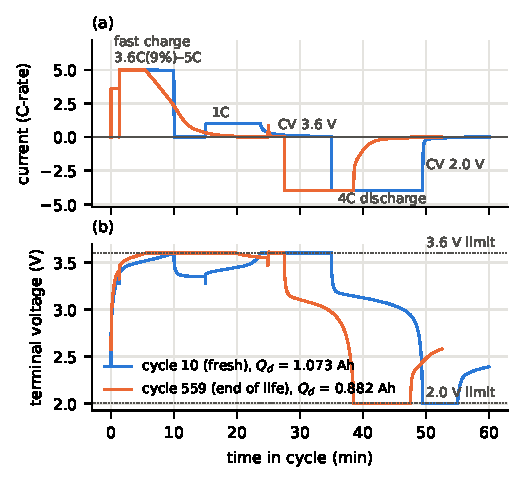
\includegraphics[width=\columnwidth]{fig_cycle}
  \caption{One cycle of cell \texttt{b2c10} when fresh and at end of life.
  (a)~Current; (b)~terminal voltage.}
  \label{fig:cycle}
\end{figure}

\textbf{Degradation.} Because the CV holds let the current decay, the
measured capacity is not limited by resistance; it falls through loss of
lithium (SEI growth, plating) and loss of graphite active material. Loss of
graphite first only shifts the voltage curve, since graphite is in excess.
When its capacity falls below the lithium inventory, lithium plates during
fast charge and the knee follows~\cite{severson2019}. Life is thus set by a
hidden margin that is used up before any capacity loss is visible.

\textbf{What $\dq$ measures.} $\dq=Q_{100}(V)-Q_{10}(V)$ is the horizontal
distance between two 4\,C discharge curves. On the flat LFP plateau a small
change in the curve gives a large shift, so $\dq$ reveals degradation that
the total capacity does not; its variance measures how unevenly the curve
has changed.

\textbf{Anode overhang.} The graphite electrode extends beyond the cathode.
Lithium stored in this overhang returns slowly during the first
cycles~\cite{severson2019}, so capacity first \emph{rises} by a few mAh
(median 3.1\,mAh; 65--80\,\% of it before cycle 10 in b1--b3). Whether the part after cycle 10
carries information is tested in Section~\ref{sec:rq3}.
